%%%%%%%%%%%%%%%%%%%%%%%%%%%%%%%%%%%%%%%%%%%%%%%%%%%%%%%%%%%%
%%%   Tracking and Analyzing The 2013 Italian Election   %%%
%%%%%%%%%%%%%%%%%%%%%%%%%%%%%%%%%%%%%%%%%%%%%%%%%%%%%%%%%%%%

\documentclass{llncs}

\newcommand{\superscript}[1]{\ensuremath{^{\textrm{#1}}}}

\usepackage{makeidx}  % allows for indexgeneration
\usepackage[hyphens]{url}
\usepackage{textcomp}
\usepackage{color}
\usepackage{listings}
\usepackage{multirow}
\usepackage{mathtools}
\usepackage{graphicx}
\usepackage{fancyvrb}
\usepackage{amsmath}
\usepackage{graphicx}
\usepackage[font=small,labelfont=bf]{caption}
\setcounter{MaxMatrixCols}{20}
\usepackage{pbox}
\usepackage{amsfonts}


% listing styles
\lstset{numbers=left, numberstyle=\tiny,basicstyle=\ttfamily\scriptsize, tabsize=2, keywordstyle=\underbar, stringstyle=\small, backgroundcolor=\color[gray]{0.94}, framexleftmargin=2pt}
\lstdefinestyle{rdfa}{numberblanklines=true, morekeywords={}}



\begin{document}
\frontmatter          % for the preliminaries
\pagestyle{headings}  % switches on printing of running heads
\mainmatter              % start of the contributions
\title{LinkedTV News \\ The 2013 Italian Election}
\titlerunning{Tracking and Analyzing The 2013 Italian Election}  % abbreviated title (for running head)

\title{LinkedTV News a companion application for newscasts}
\author{Michiel Hildebrand\inst{1}, Lilia Perez Romero\inst{1}, Jos\'e Luis Redondo Garc\'ia\inst{2}, Rapha\"el Troncy\inst{2}}
\institute{CWI, Amsterdam, The Netherlands, \\
\email{\{M.Hildebrand, L.Perez\}@cwi.nl}
\and
EURECOM, Sophia Antipolis, France, \\
\email{\{redondo, raphael.troncy\}@eurecom.fr}
}


\maketitle              % typeset the title of the contribution

%%%%%%%%%%%%%%%%%%
%%%  Abstract  %%%
%%%%%%%%%%%%%%%%%%

\begin{abstract}
Describing multimedia content in general and TV programs in particular is a hard problem. Relying on subtitles to extract named entities that can be used to index fragments of a program is a common method. However, this approach is limited to what is being said in a program and written in a subtitle, therefore lacking a broader context. Furthermore, this type of index is restricted to a flat list of entities. In this paper, we combine the power of non-structured documents with structured data coming from DBpedia to generate a much richer, context aware metadata of a TV program. We demonstrate that we can harvest a rich context by expanding an initial set of named entities detected in a TV fragment. We evaluate our approach on a TV news show.

\keywords{Television, Visual Summarization, Topic Generation}
\end{abstract}

%%%%%%%%%%%%%%%%%%%%%%%%%
%%%  1. Introduction  %%%
%%%%%%%%%%%%%%%%%%%%%%%%%

\section{Introduction}

People consume news from multiple sources, such as television, Web, radio and newspaper. Typically the activities using these sources are independent~\cite{}. For example, we watch the newscast on TV at a fixed time of the day to get an overview of the main news. We use the Web to keep track of the News throughout the day, and when we have more time to spare we actively browse the Web to explore the news items that we are interested in. At one hand this separation is natural as the activities have different characteristics and are integrated into our lifes in our way. At the other hand the different sources can complement each other and when consumed as such will enrich our news experience. The problem is that in practice it is difficult to manually link the different activities together. How often did you think of something you wanted to lookup on the Web while watching a newscast, but didn't, or while browsing the Web could not remember that one news item you saw on TV and wanted to explore further? 

We present an application that links the activities of watching the news on TV and looking up information on the Web. The application is the outcome of a process of user-centered design to gather information needs, iteratively design the prototype and evaluate the usability. The application supports two types of information needs: (i) looking up factual information about persons, locations, organisations and concepts occuring in the newscast, and (ii) exploring more indepth information about a news item. An important design consideration to realize support for these types of information needs was to respect the intrinsic user behavior associated with watching TV, lean back, and browsing the Web, lean forward. As a result the application operates in two modes. 

In the passive mode the application operates as a second screen that is synced with the TV program. This mode supports the user with looking up factual information by presenting timed slides about the entities that occur in the news. As this mode requiers no interaction it unobtrusevely complements the lean back TV viewing experience. In addition, the passive mode provides functionality to bookmark news items. This one click interaction forms the bridge to the active mode of the application. 

In the active mode the user actively explores a specific news item. In this mode the application contains articles from the Web that are related to the news item in different dimensions. The dimension, such as articles from different news sources, opionion articles and a timeline of past events, are intended to support the specific user information needs that were identified in the study. While it is possible to use the active mode during the broadcast, this will disrupt the passive TV viewing experience. By first bookmarking the news item the user can come back to the application at a more appropriate time to start or continue the exploration.

%%%%%%%%%%%%%%%%%%
%%%  Annotating TV News  %%%
%%%%%%%%%%%%%%%%%%

\section{Annotating TV News}
To reconstruct the semantic context associated with one particular news video, we extract the main concepts and entities from the subtitles and explain how they are related to each other. The complete processing workflow takes as input the textual transcript of a multimedia resource illustrating an event, as well as the start and end date for which that particular event is considered. We assume that this event has a minimal presence and coverage on the Web to ensure that the subsequent data mining techniques can collect sufficient data to reconstruct the event's context. 

For each news item, we perform named-entity recognition over the corresponding subtitles using the NERD framework~\cite{Rizzo2012b}. In our experiment, the language of the videos is English but NERD supports other languages. The output of this phase is a collection of entities annotated using the NERD Ontology\footnote{\fontsize{8pt}{1em}\selectfont \url{http://nerd.eurecom.fr/ontology/nerd-v0.5.n3}}, that comes with a first relevance score obtained from the extractors which have been used. This set includes a list of ranked entities that are explicitly mentioned during the video. Other entity based video annotation tools~\cite{yunjia2013} stop at this point even when entities that can be relevant for the viewer in the context of the event are still missing. We tackle this problem by extending this first list of concepts via the entity expansion component.

The set of entities obtained from a traditional named entity extraction operation is normally insufficient and incomplete for expressing the context of a news event. Sometimes, some entities spotted over a particular document are not disambiguated because the textual clues surrounding the entity are not precise enough for the name entity extractor, while in other cases, they are simply not mentioned in the transcripts while being relevant for understanding the story. We perform the a process named entity expansion operation, which relies on the idea of retrieving and analyzing additional documents from the Web where the same event is also described. By increasing the size of set of documents to analyse, we increase the completeness of the context and the representativeness of the list of entities, reinforcing relevant entities and finding new ones that are potentially interesting inside the context of that news item.

The entire logic is illustrated in in Figure~\ref{fig:namedEntityExpansion} and consists mainly in (1) building an appropriate search query from the original set of entities, (2) retrieving additional documents about the same news event, and (3) analyzing them for providing a more complete and better ranked set of final entities, as illustrated in Figure~\ref{fig:namedEntityExpansion}.

\begin{figure}[h!]
\centering
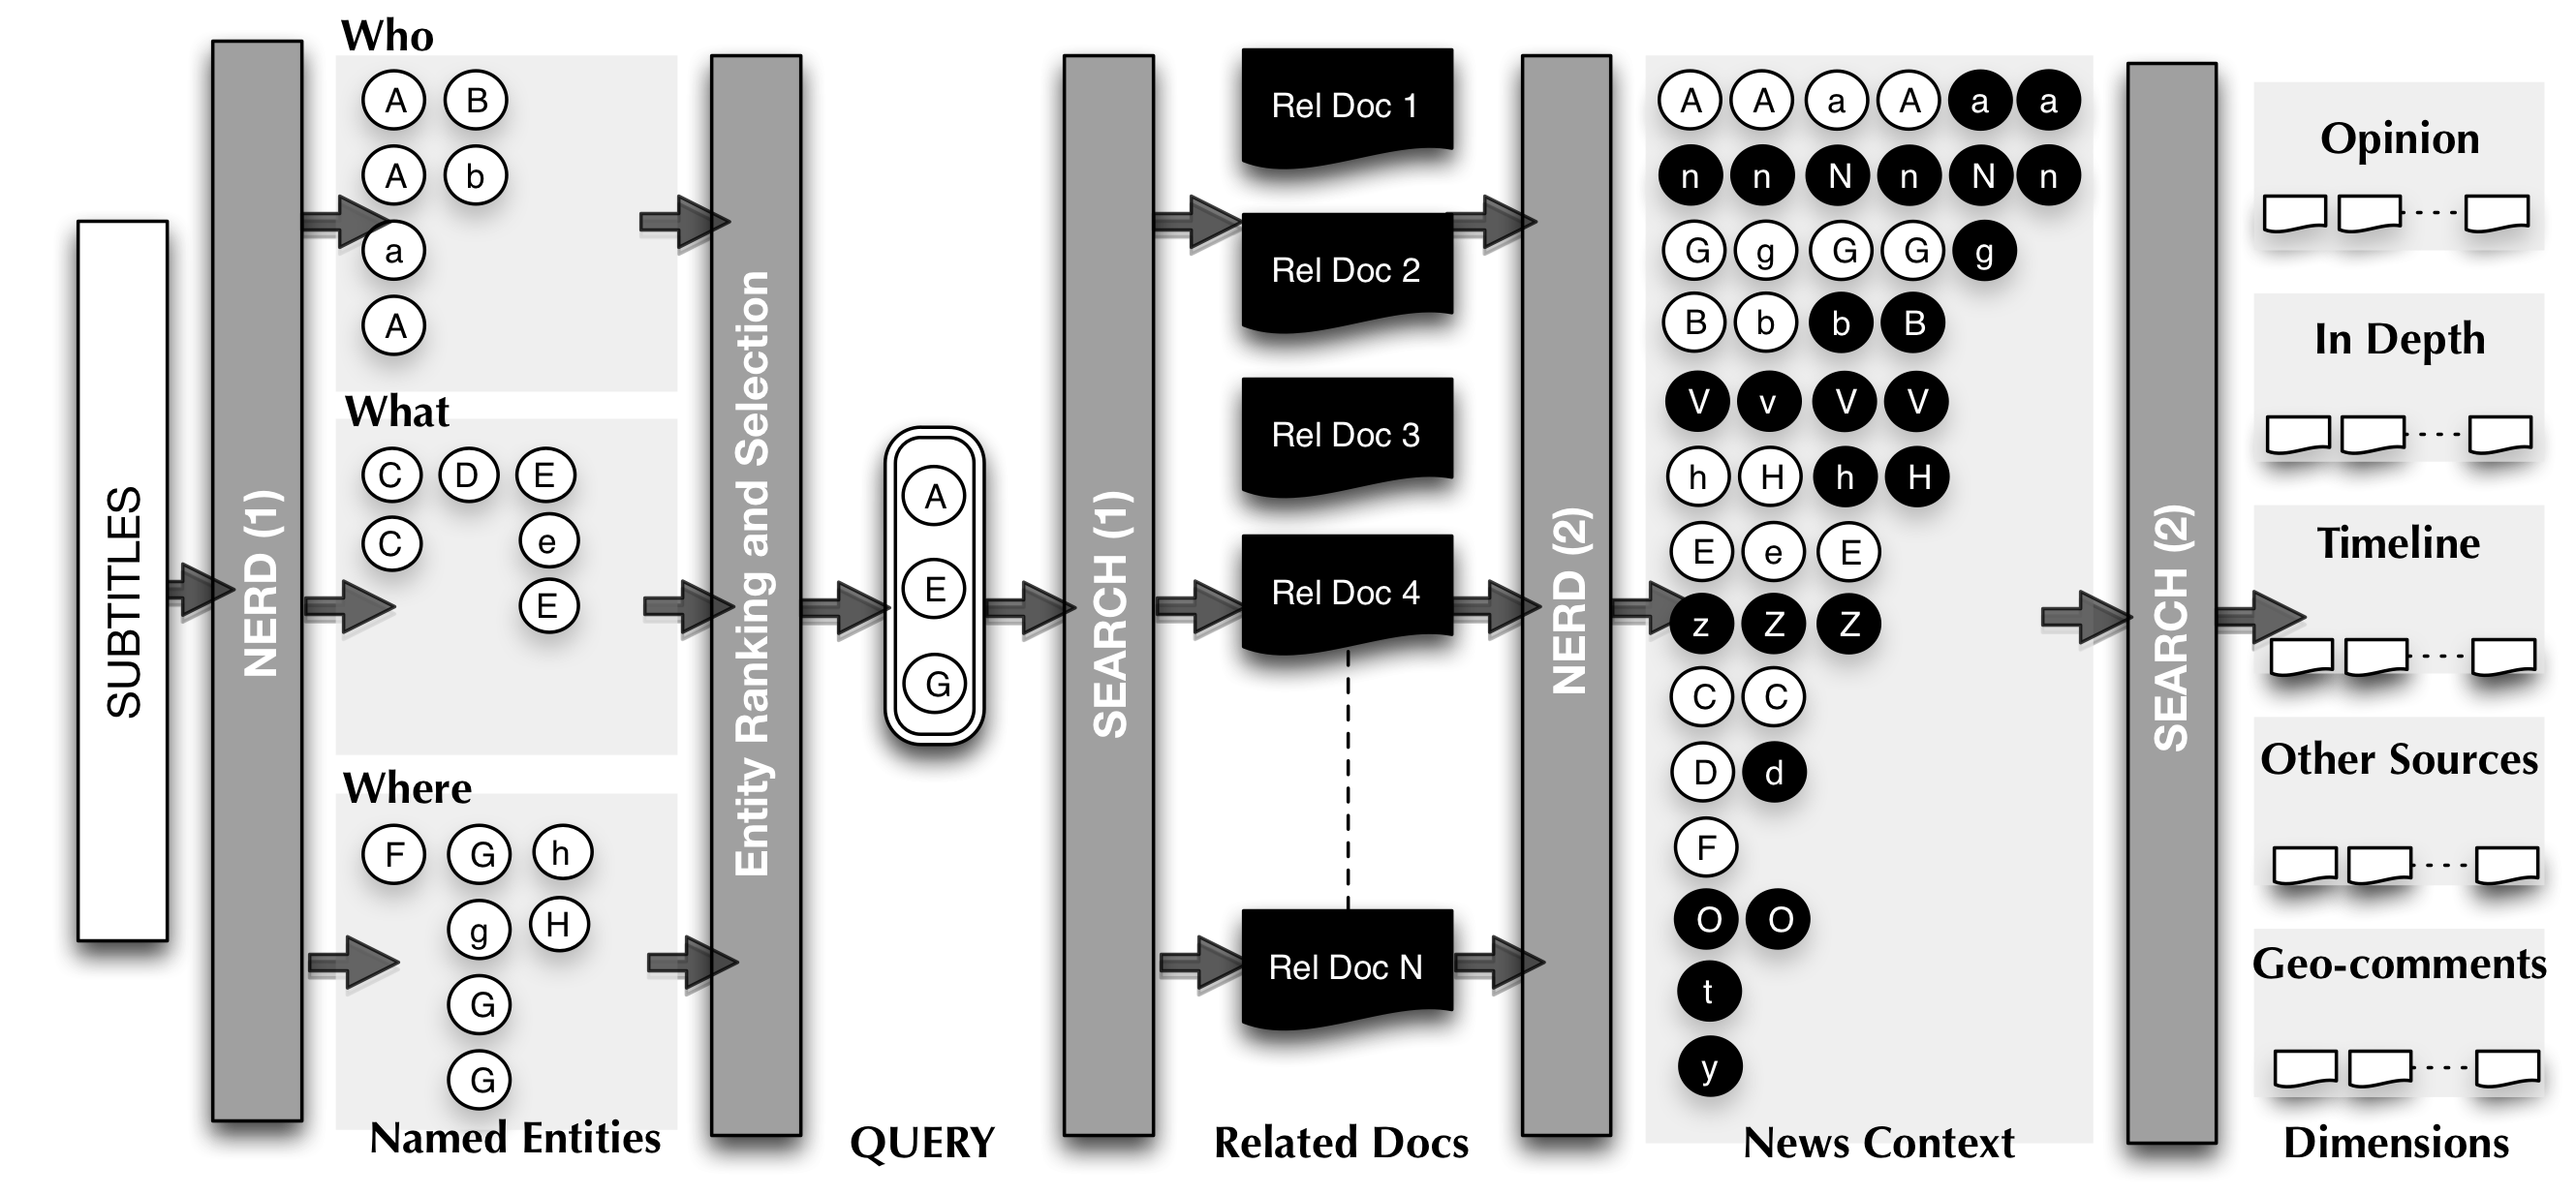
\includegraphics[width=0.6\textwidth]{figure/ExpansionDiagram}
\caption{Schema of Named Entity Expansion Algorithm.}
\label{fig:namedEntityExpansion}%\end{figure}
\end{figure}

The \emph{Five W's} is a popular concept of information gathering in journalistic reporting. It captures the main aspects of a story: who, when, what, where, and why~\cite{LiJia2007}. We try to represent the news item in terms of four of those five W's (who is involved in the event, where the event is taking place, what the event is about, and when it has happened) in order to generate a query that retrieves documents associated to the same event.

First, the original entities are mapped to the NERD Core ontology, which considers 10 main classes: Thing, Amount, Animal, Event, Function, Organization, Location, Person, Product and Time. From those ten different categories, we generalize to three classes: the Who from \url{nerd:Person} and \url{nerd:Organization}, the Where from \url{nerd:Location}, and the What from the rest of NERD types after discarding \url{nerd:Time} and \url{nerd:Amount}. The When or so-called temporal dimension does not need to be computed since it is considered to be provided by the video publisher.

After generating the three sets of entities, the next step consist in ranking them in relevance according to a weighted sum of two different dimensions: their frequency in the transcripts and their former relevance scores coming from the named entity extractors. We have defined the function \emph{filterEntities(S)} for selecting the $n$ entities inside the set of entities $S$ whose relative relevance falls into the upper quarter of the interval.

The final query is a pair where \textit{textQuery} is the result of concatenating the labels of the most relevant entities in the sets Who, What, Where in that particular order, and $t$ the time period dimension. This query generation is depicted in the upper part of Figure~\ref{fig:namedEntityExpansion}.

\subsubsection{Document Retrieval}
Once $\text{Query}_{Event}$ is built out of the original set of named entities, it will be ready to be injected into a document search engine where additional descriptions about the news event can be found. In this situation, the kind of query generated in the previous step and the search engine chosen should be closely tied in order to maximize the quality of the obtained results. The different behavior of search engines make some alternatives more suitable than others for certain kinds of events. The way the resulting documents change in the search engines for a particular kind of event is a research question that will not be studied in this paper.

In this paper, we rely on the Google Search REST API service\footnote{\fontsize{8pt}{1em}\selectfont  \url{http://ajax.googleapis.com/ajax/services/search/web?v=1.0}} by launching a query with the text \textit{textQuery}. Due to quota restrictions imposed by Google, the maximum number of retrieved document is set to 30. However, as shown in the evaluation described in the Section~\ref{sec:evaluation}, this is enough for significantly extending the initial set of entities directly spotted by NERD.

Concerning the temporal dimension, we only keep the documents published in the time period $t+t_{e}$. We increase the original event period in $t_{e}$ because documents concerning a news event are not always published during the time of the action is taking place but some hours or days after. The value of $t_{e}$ depends on many factors such as the nature of the event itself (whether it is a brief appearance in a media, or part of a longer story with more repercussion) or the kind of documents the search engine is indexing (from very deep and elaborated documents that need time to be published, to short post quickly generated by users). Based on the simple assumption that that the longer is an event, and the longer it is likely to generate buzzes, we approximated  $t_{e} = t$ which means that we also consider document published during the course of an event.

The middle part of Figure~\ref{fig:namedEntityExpansion} shows this process. The query is input in the search engine in order to retrieve other documents that report on the same event discussed in the original video. Those documents (colored in black in the Figure~\ref{fig:namedEntityExpansion}) will be further processed to increase the size of the collection and get additional insights about the news item.

\subsubsection{Entity Clustering}
In this phase, the additional documents which have just been retrieved are now processed and analyzed in order to extend and re-rank the original set of entities and consequently get a better insight about the event. Since most of the resources retrieved are Web pages, HTML tags and other annotations are removed, keeping only the main textual information. This plain text is then analyzed by the NERD framework in order to extract more named entities.

In order to calculate the frequency of a particular resource within the entire corpora, we group the different appearances of the same instance and check their cardinality. This is not a trivial task since the same entity can appear under different text labels, contain typos or have different disambiguation URL's pointing to the same resource. We performed a centroid-based clustering operation over the instances of the entities. We considered the centroid of a cluster as the entity with the most frequent disambiguation URL's that also have the most repeated labels. As distance metric for comparing pairs of entities, we applied strict string similarity over the URL's, and in case of mismatch, the Jaro-Winkler string distance~\cite{winkler2006overview} over the labels. The output of this phase is a list of clusters containing different instances of the same entity.

\subsubsection{Entity Ranking}
The final step of the expansion consists of ranking the different named entities obtained so far. To create this ordered list, we assigned a score to every entity according to the following features: relative frequency in the transcripts of the event video; relative frequency over the additional document; and average relevance according to the named entity extractors. The three dimensions are combined via a weighted sum where the frequency in the video subtitles has a bigger impact, followed by the frequency on the searched documents and the relevance from the extractors. The final output of the entity expansion operation is a list of entities together with their ranking score and the frequency in both the main video and in the collected documents retrieved from the search engine.

Entities with a higher $relScore_{i}$ in the final classification are considered more representative for describing the context than the original entities. Furthermore, we observe that:
\begin{itemize}
  \item The bigger the sample size, and the better becomes the ranking. Entities appearing repeatedly in the additional documents will be promoted while those appearing rarely will be pushed back to the end of the list.
  \item Entities that originally have not been disambiguated can now have their corresponding URL if any of the similar instances appearing in the additional documents provide a link to a Web resource. The same occurs with incomplete or misspelled labels.
  \item Finally, some entities not spotted in the original transcripts but important in the context of the event are now included in the list of relevant items since they have been extracted from the collected documents.
\end{itemize}

%%%%%%%%%%%%%%%%%%%%%%%
%%%  3. Visualization of Entities  %%%
%%%%%%%%%%%%%%%%%%%%%%%

\section{Visualization: the case of Edward Snowden}
\label{sec:usecase}

%%%%%%%%%%%%%%%%%%%%%%%
%%%  4. Discussion  %%%
%%%%%%%%%%%%%%%%%%%%%%%

\section{Discussion}
\label{sec:discussion}
During the first day (February 26th), no party was a clear winner of the election, but Monti's defeat stood out. International newspapers reported about it, fueling the discussion on social platforms. Similarly, the 27th is the day after Bersani's speech. His words about the dramatic situation became popular and viral. Another example of the usefulness of our automatic approach is the day 28th, when the world started to investigate about \textit{The cult of Silvio Berlusconi} and the reaction from the crowd (catched by our storyboard) is immediately depicted. On March 1st, the Italian president visited Germany and met the German chancellor Merkel to discuss, amongst others, the Italian elections. On March 2nd, Grillo claimed no collaboration with any party. Grillo is the \textit{Movimento 5 Stelle} leader, incorrectly identified by our approach as \textit{Stelle}. This is due to the lack of knowledge of our entity spotter. In the same day, both a famous Italian talk show and an Economist article triggered a lot of discussion about the current Italian situation, Grillo and Berlusconi. Again, Grillo and Berlusconi were trending. On March 3rd, the kick-off meeting of the Beppe Grillo's party took place. The main action lines were rejecting possible alliance with any parties and especially with the Bersani's party.

The election use case showed that our approach provides useful insights about events while leveraging from the crowd. In a wide sense, it provides a snapshot of how the crowd is experiencing an event. We focus on generating visual summaries in order to illustrate those phenomena. We argue that the need of human intervention in the collection and interpretation processes has been drastically reduced. The different clustering operations and the user interface give to the user a tool for interpreting the story, even if some background knowledge about the event is required. Although the crowd talked about the same main entities reported by daily newspapers, we observe that different satirical expressions for talking about politics are used. Actually, numerous images and posts are biased towards being satirical. Tracking and understanding an event from social data should also include the popularity of microposts. We have planned to use this measure as an additional mean for weighting the importance of a social peak. We will further demonstrate how this tool can been used to generate visual summaries of highly viral memes such as \emph{Harlem Shake}.

%%%%%%%%%%%%%%%%%%%%%%%%%
%%%  Acknowledgments  %%%
%%%%%%%%%%%%%%%%%%%%%%%%%

\section*{Acknowledgments}
This work was partially supported by the European Union's 7th Framework Programme via the project LinkedTV (GA 287911).

%%%%%%%%%%%%%%%%%%%%%%
%%%  Bibliography  %%%
%%%%%%%%%%%%%%%%%%%%%%
\bibliographystyle{abbrv}
\bibliography{EnrichedTVNews}

\end{document}
